%%%%%%%%%% Glossar %%%%%%%%%%%%%%%%
\newglossaryentry{gDB_Anwendungsverantwortliche(Admin)}{
	name={Anwendungsverantwortliche},
	description={
		Diese Person hat die Projekt/Stakeholder und Entwicklungsverantwortung. Sie erfasst die Anforderungen aus dem Geschäftsbereich. Die Rolle wird der Person zu gewiessen, welche die \textit{Entwicklungsumgebung} über das Digitalportal bestellt.
	\begin{figure}[H]
		\centering
		
\includegraphics[scale = 0.3]{attachment/x_glossar/Scc003}
	\end{figure}
	}
}

\newglossaryentry{gDB_Enviromentverantwortliche(Maker)}{
	name={Anwendungsentwicklerin},
	description={
		Diese Person, wird durch die \gls{gDB_Anwendungsverantwortliche(Admin)}, in der Entwicklungsumgebung der Maker-Rolle zugewiesen. Diese ist für die Entwicklung der Anwendung oder des Flows zuständig.
	\begin{figure}[H]
		\centering
		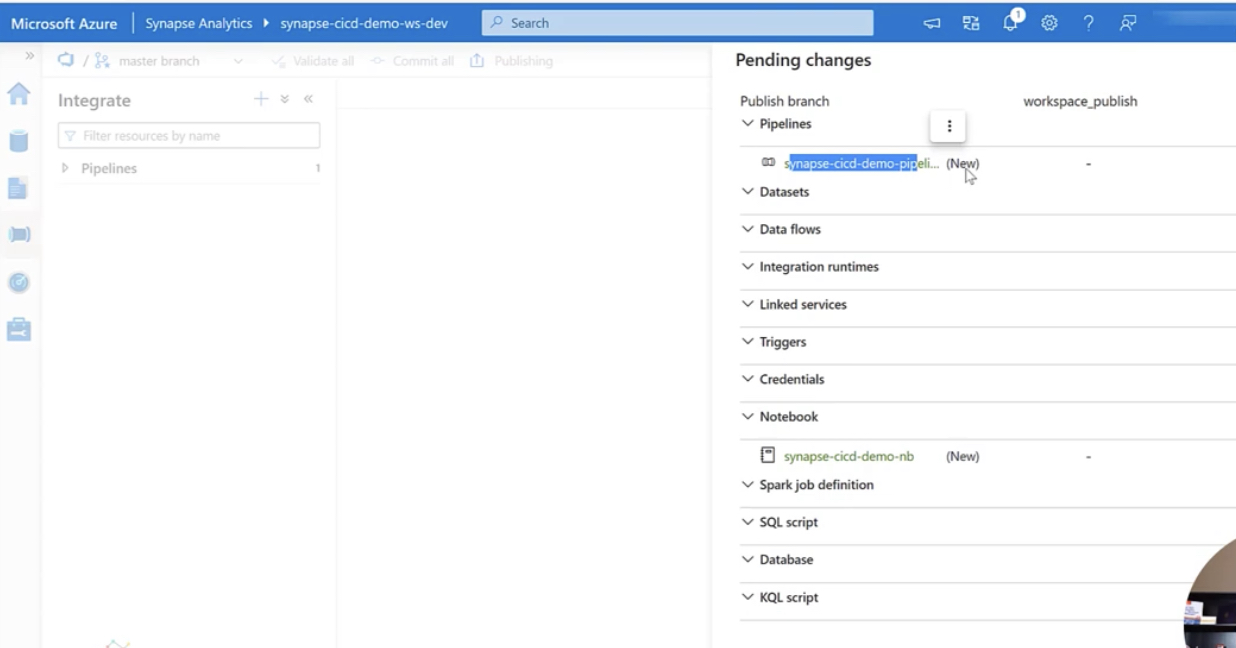
\includegraphics[scale = 0.3]{attachment/x_glossar/Scc151}
	\end{figure}
	}
}

\newglossaryentry{gDB_Enviromentverantwortliche(Admin)}{
	name={Enviromentverantwortliche/Mutli-Stage Verantwortliche},
	description={
			Diese Person hat die DB-Goverance und Prozessverantwortung. Sie überwacht die Hostung verschiedener Applikationen/ Flows in der Produktionsumgebung. Die Rolle wird der Person zu gewiessen, welche die \textit{Multi-Stage Umgebung} über das Digitalportal bestellt.
	\begin{figure}[H]
		\centering
		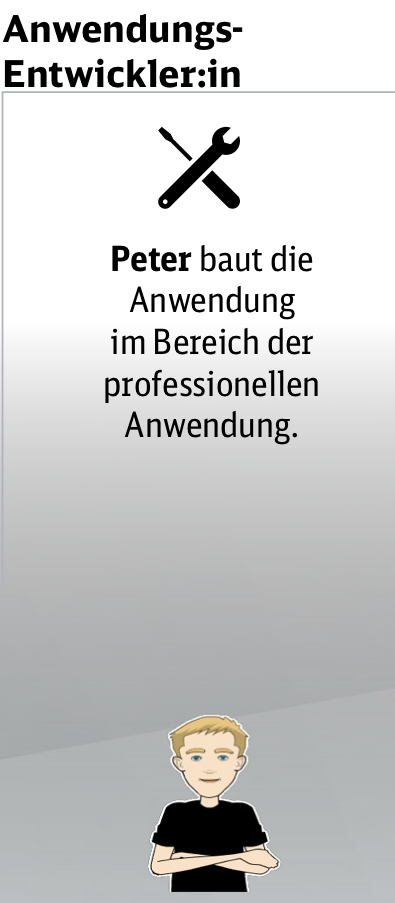
\includegraphics[scale = 0.3]{attachment/x_glossar/Scc001}
	\end{figure}
	}
}